\documentclass[a4paper,12pt]{article}
\usepackage{amssymb} % needed for math
\usepackage{amsmath} % needed for math
\usepackage[utf8]{inputenc} % this is needed for german umlauts
\usepackage[ngerman]{babel} % this is needed for german umlauts
\usepackage[T1]{fontenc}    % this is needed for correct output of umlauts in pdf
\usepackage[margin=2.5cm]{geometry} %layout
\usepackage{booktabs}
\usepackage{tabularx}

% this is needed for forms and links within the text
\usepackage{hyperref}

% glossar, see http://en.wikibooks.org/wiki/LaTeX/Glossary
% has to be loaded AFTER hyperref so that entries are clickable
\usepackage[nonumberlist]{glossaries} 

% The following is needed in order to make the code compatible
% with both latex/dvips and pdflatex.
\ifx\pdftexversion\undefined
\usepackage[dvips]{graphicx}
\else
\usepackage[pdftex]{graphicx}
\DeclareGraphicsRule{*}{mps}{*}{}
\fi

\makeglossary

\newcommand{\authorName}{Dustin Spallek, Rene Kretschmer, Christof Rode, Jana Wengenroth, Malte Scheller, Daniel Schruhl}
\newcommand{\projektName}{Anbieter Informations Management}
\newcommand{\tags}{\authorName, Pflichtenheft}
\newcommand{\glossarName}{Glossar}
\title{\projektName~(Pflichtenheft)}
\author{Dustin Spallek, Rene Kretschmer, Christof Rode, Jana Wengenroth, \\Malte Scheller, Daniel Schruhl}
\date{\today}

\hypersetup{
  pdfauthor   = {\authorName},
  pdfkeywords = {\tags},
  pdftitle    = {\projektName~(Pflichtenheft)}
} 
 
\newcommand\addrow[2]{#1 &#2\\ }

\newcommand\addheading[2]{#1 &#2\\ \hline}
\newcommand\tabularhead{\begin{tabular}{lp{13cm}}
\hline
}

\newcommand\addmulrow[2]{ \begin{minipage}[t][][t]{2.5cm}#1\end{minipage}% 
   &\begin{minipage}[t][][t]{8cm}
    \begin{enumerate} #2   \end{enumerate}
    \end{minipage}\\ }

\newenvironment{usecase}{\tabularhead}
{\hline\end{tabular}}

\begin{document}
 \pagenumbering{roman}
 \begin{titlepage}
\maketitle
\thispagestyle{empty} % no page number

\begin{verbatim}












\end{verbatim}


  \begin{tabular}[t]{ll}
	Projekt:       & \quad \projektName \\[1.2ex]
  \end{tabular}

\begin{tabularx}{\textwidth}{|l|l|X|}
\hline
\textbf{Version} & \textbf{Datum} & \textbf{Autor(en)} \\
\hline
\hline
1.0 & 19.09.2016 & \authorName \\
2.0 & 10.10.2016 & \authorName \\
\hline
\end{tabularx}
\end{titlepage}
         % Deckblatt.tex laden und einfügen
 \setcounter{page}{2}
 \tableofcontents          % Inhaltsverzeichnis ausgeben
 \clearpage
 \pagenumbering{arabic}

\section{Lizenz}

 
\section{Zielbestimmung}

Es soll ein Microservice erstellt werden, um die vorhandenen Anbieter und Produktdaten anzureichern.

\subsection{Musskriterien}
\begin{usecase}
  \addheading{Nummer}{Beschreibung} 
  \addrow{/MK10/}{User können sich anmelden}
  \addrow{/MK20/}{User können sich abmelden}
  \addrow{/MK30/}{User können ihre Anbieterdaten bearbeiten}
  \addrow{/MK40/}{User können ihre Produktdaten bearbeiten}
  \addrow{/MK50/}{Dateien können in einer Dateiverwaltung hinzugefügt werden}
  \addrow{/MK60/}{Dateien können in einer Dateiverwaltung gelöscht werden}
  \addrow{/MK70/}{Dateien können in einer Dateiverwaltung ersetzt werden und die
   Verlinkungen in den Texten bleiben für die Dateien erhalten}
  \addrow{/MK80/}{Alle im System gespeicherten Daten müssen über eine Schnittstelle erreichbar sein}
  \addrow{/MK90/}{Es muss möglich sein über eine externe Konfigurations-Datei gewisse Beschränkungen vorzunehmen (siehe Produktdaten)}
\end{usecase}

\subsection{Wunschkriterien}
\begin{usecase}
  \addheading{Nummer}{Beschreibung} 
  \addrow{/WK10/}{Dateien können per Drag and Drop in der Ordnung verschoben werden}
  \addrow{/WK20/}{Die eingebaute Textbearbeitung unterstützt das Einfügen von mit Word formatierten Texten}
  \addrow{/WK30/}{Das System soll per Docker deployable gemacht werden}
\end{usecase}

\subsection{Abgrenzungskriterien}
\begin{usecase}
  \addheading{Nummer}{Beschreibung} 
  \addrow{/AK10/}{Das Programm beinhaltet kein Authentifizierungs System}
  \addrow{/AK20/}{Es können keine neuen Produkte über das System angelegt werden}
  \addrow{/AK30/}{Es können keine Produkte über das System gelöscht werden}
  \addrow{/AK40/}{Es können keine Anbieter über das System gelöscht werden}
  \addrow{/AK50/}{Es können keine neuen Anbieter über das System angelegt werden}
\end{usecase}


\section{Produkteinsatz}
Der Microservice soll in die Infrastruktur von Symphony eingegliedert werden, um für Anbieter die Funktion der Anreicherung ihrer Produktdaten zu ermöglichen.

\subsection{Zielgruppe}
Unsere Zielgruppe sind alle Mitarbeiter der Anbieter, die einen Zugang zum System haben.

\subsection{Anwendungsbereiche}
Administrative Anwendungsbereiche zur Verwaltung und Anreicherung der Anbieter und Produktdaten.

\section{Produktumgebung}
\subsection{Software}
\subsection{Hardware}
\subsection{Orgware}
\subsection{Produktschnittstellen}



\section{Funktionale Anforderungen}
\subsection{Login}\label{login}
Der Benutzer kann sich anhand seiner Symphony Zugangsdaten am System anmelden.

\subsubsection{Vorbedingung}\label{vorbedingung}

\begin{itemize}
\item
  Benutzer ist nicht angemeldet
\item
  Benutzer hat einen gültigen Account
\item
  Schnittstellen sind verfügbar
\end{itemize}

\subsubsection{Nachbedingung}\label{nachbedingung}

\begin{itemize}
\item
  es findet eine Weiterleitung auf den geschützten Bereich statt
\end{itemize}

\subsubsection{Benutzer Aktion}\label{benutzer-aktion}

\begin{itemize}
\item
  Benutzer gibt seine Anmeldedaten (Benutzername, Passwort) ein
\item
  drückt auf Login/Enter
\end{itemize}

\subsubsection{System Aktion}\label{system-aktion}

\begin{itemize}
\item
  die Anmeldedaten werden vom Authentifizierungsserver validiert
\item
  das System ruft Produkt- und Anbieterinformationen ab
\end{itemize}

\subsubsection{Fehlerfälle}\label{fehlerfalle}

\begin{itemize}
\item
  Anmeldedaten sind falsch / kein Konto vorhanden -\textgreater{}
  Meldung: Falsche Daten eingegeben
\item
  Authentifizierungsservice nicht erreichbar -\textgreater{} Meldung:
  Technisches Problem, versuchen Sie es noch einmal (einloggen ist nicht
  möglich)
\item
  Produktservice nicht erreichbar -\textgreater{} Meldung: Technisches
  Problem, versuchen Sie es noch einmal (einloggen ist nicht möglich)
\end{itemize}

\subsubsection{Erweiterung}\label{erweiterung}
Keine weiteren Angaben.

\subsubsection{Abgrenzung}\label{abgrenzung}

\begin{itemize}
\item
  Kein Passwort verändern
\item
  Kein Passwort vergessen
\item
  Kein Account anlegen
\item
  Kein Benutzer merken
\end{itemize}

\subsection{Logout}\label{logout}
Der Benutzer meldet sich vom System ab.

\subsubsection{Vorbedingung}\label{vorbedingung-1}

\begin{itemize}
\item
  Benutzer ist angemeldet
\end{itemize}

\subsubsection{Nachbedingung}\label{nachbedingung-1}

\begin{itemize}
\item
  es findet eine Weiterleitung auf eine vom Kunden gewünschte Seite
  statt
\end{itemize}

\subsubsection{Benutzer Aktion}\label{benutzer-aktion-1}

\begin{itemize}
\item
  drückt auf Logout
\end{itemize}

\subsubsection{System Aktion}\label{system-aktion-1}

\begin{itemize}
\item
  Logout wird an den Authentifizierungsservice mit den Benutzerdaten
  geschickt
\end{itemize}

\subsubsection{Fehlerfälle}\label{fehlerfalle-1}
Keine weiteren Angaben.

\subsubsection{Erweiterung}\label{erweiterung}
Keine weiteren Angaben.

\subsubsection{Abgrenzung}\label{abgrenzung}

\begin{itemize}
\item
  Authentifizierungsservice nicht erreichbar -\textgreater{} Meldung:
  Technisches Problem, versuchen Sie es noch einmal (ausloggen ist nicht
  möglich)
\end{itemize}

\clearpage

\subsection{Bearbeitung der Kurzbeschreibung}
Der Benutzer bearbeitet die Anbieter Kurzbeschreibung bzw. die Produkt Kurzbeschreibung.
\subsubsection{Vorbedingung}

\begin{itemize}
\item
  Benutzer ist angemeldet
\end{itemize}

\subsubsection{Nachbedingung}\label{nachbedingung-2}

\begin{itemize}
\item
  Benutzer wird über seine durchgeführten Aktionen informiert
  (verwerfen, speichern)
\item
  Daten werden in der Datenbank persistiert
\end{itemize}

\subsubsection{Benutzer Aktion}\label{benutzer-aktion-2}

\begin{itemize}
\item
  Benutzer wählt links im Menü seinen zu bearbeitenden Punkt (Anbieter
  oder Produkt) aus
\item
  Benutzer bearbeitet den Text der Kurzbeschreibung
\item
  Benutzer klickt auf speichern / verwerfen (siehe Erweiterung)
\end{itemize}

\subsubsection{System Aktion}\label{system-aktion-2}

\begin{itemize}
\item
  System speichert die entsprechenden Daten in der Datenbank
\end{itemize}

\subsubsection{Fehlerfälle}\label{fehlerfalle-2}

\begin{itemize}
\item
  Eingaben sind zu lang (Felder sind begrenzt) -\textgreater{} Feld wird
  rot, Meldung: Zu lang!
\item
  Eingaben sind ungültig (z.B.: HTML in Kurzbeschreibung)
  -\textgreater{} Feld wird rot, Meldung: Ungültige Eingabe!
\item
  Felder sind leer -\textgreater{} Feld wird rot, Meldung: Bitte füllen
  Sie alle nötigen Felder aus
\end{itemize}

\subsubsection{Erweiterung}\label{erweiterung-2}

\begin{itemize}

\item
  Beim Verwerfen und Speichern wird die Maske nicht verlassen
\item
  Beim Verwerfen werden alle ungespeicherten Daten verworfen
\item
  Benutzer wird über seine durchgeführten Aktionen informiert
  (verwerfen, speichern)
\end{itemize}

\subsubsection{Abgrenzung}\label{abgrenzung-2}

\begin{itemize}

\item
  Das Speichern der Daten kann nur durchgeführt werden, wenn der
  Benutzer auf Speichern klickt. Ungespeicherte Änderungen gehen
  verloren, wenn die Seite z.B. aktualisiert oder verlassen wird
\end{itemize}

\clearpage

\subsection{Bearbeitung der Detailbeschreibungen}
Der Benutzer bearbeitet Anbieter bzw. Produkt Detailbeschreibungen.

\subsubsection{Vorbedingung}\label{vorbedingung-3}

\begin{itemize}

\item
  Benutzer ist angemeldet
\end{itemize}

\subsubsection{Nachbedingung}\label{nachbedingung-3}

\begin{itemize}

\item
  Benutzer wird über seine durchgeführten Aktionen informiert
  (verwerfen, speichern)
\item
  Daten werden in der Datenbank persistiert
\end{itemize}

\subsubsection{Benutzer Aktion}\label{benutzer-aktion-3}

\begin{itemize}

\item
  Benutzer wählt links im Menü seinen zu bearbeitenden Punkt (Anbieter
  oder Produkt) aus
\item
  Benutzer bearbeitet den Text der Detailbeschreibung
\item
  Benutzer klickt auf speichern / verwerfen (siehe Erweiterung)
\end{itemize}

\subsubsection{System Aktion}\label{system-aktion-3}

\begin{itemize}

\item
  System speichert die entsprechenden Daten in der Datenbank
\end{itemize}

\subsubsection{Fehlerfälle}\label{fehlerfalle-3}

\begin{itemize}

\item
  Eingaben sind zu lang (Felder sind begrenzt) -\textgreater{} Feld wird
  rot, Meldung: Zu lang!
\item
  Eingaben sind ungültig (z.B.: HTML in Kurzbeschreibung)
  -\textgreater{} Feld wird rot, Meldung: Ungültige Eingabe!
\item
  Felder sind leer -\textgreater{} Feld wird rot, Meldung: Bitte füllen
  Sie alle nötigen Felder aus
\end{itemize}

\subsubsection{Erweiterung}\label{erweiterung-3}

\begin{itemize}

\item
  Beim Verwerfen und Speichern wird die Maske nicht verlassen
\item
  Beim Verwerfen werden alle ungespeicherten Daten verworfen
\item
  Benutzer wird über seine durchgeführten Aktionen informiert
  (verwerfen, speichern)
\end{itemize}

\subsubsection{Abgrenzung}\label{abgrenzung-3}

\begin{itemize}

\item
  Das Speichern der Daten kann nur durchgeführt werden, wenn der
  Benutzer auf Speichern klickt. Ungespeicherte Änderungen gehen
  verloren, wenn die Seite z.B. aktualisiert oder verlassen wird
\end{itemize}

\clearpage

\subsection{Bearbeitung des Hauptbildes}
Der Benutzer bearbeitet das Anbieter bzw. Produkt Hauptbild.

\subsubsection{Vorbedingung}\label{vorbedingung-4}

\begin{itemize}

\item
  Benutzer ist angemeldet
\end{itemize}

\subsubsection{Nachbedingung}\label{nachbedingung-4}

\begin{itemize}

\item
  Benutzer wird über seine durchgeführten Aktionen informiert
  (verwerfen, speichern)
\end{itemize}

\subsubsection{Benutzer Aktion}\label{benutzer-aktion-4}

\begin{itemize}

\item
  Benutzer wählt links im Menü seinen zu bearbeitenden Punkt (Anbieter
  oder Produkt) aus
\item
  Benutzer klickt auf Hauptbild auswählen
\item
  Benutzer wählt aus der Liste von Dateien ein Hauptbild aus und
  bestätigt mit OK
\item
  Benutzer klickt auf speichern / verwerfen (siehe Erweiterung)
\end{itemize}

\subsubsection{System Aktion}\label{system-aktion-4}

\begin{itemize}

\item
  System speichert die entsprechenden Auswahl in der Datenbank
\end{itemize}

\subsubsection{Fehlerfälle}\label{fehlerfalle-4}
Keine weiteren Angaben.

\subsubsection{Erweiterung}\label{erweiterung-4}

\begin{itemize}

\item
  Beim Verwerfen und Speichern wird die Maske nicht verlassen
\item
  Beim Verwerfen werden alle ungespeicherten Daten verworfen
\item
  Benutzer wird über seine durchgeführten Aktionen informiert
  (verwerfen, speichern)
\end{itemize}

\subsubsection{Abgrenzung}\label{abgrenzung-4}

\begin{itemize}

\item
  Das Speichern der Daten kann nur durchgeführt werden, wenn der
  Benutzer auf Speichern klickt. Ungespeicherte Änderungen gehen
  verloren, wenn die Seite z.B. aktualisiert oder verlassen wird
\item
  Für die Hauptbild Auswahl stehen nur Bilddateien zur Verfügung (keine
  PDF)
\end{itemize}

\subsection{Bearbeitung der Galerie}
Der Benutzer fügt Dateien zur Anbieter bzw. Produkt Galerie hinzu.

\subsubsection{Vorbedingung}\label{vorbedingung-5}

\begin{itemize}

\item
  Benutzer ist angemeldet
\end{itemize}

\subsubsection{Nachbedingung}\label{nachbedingung-5}

\begin{itemize}

\item
  Benutzer wird über seine durchgeführten Aktionen informiert
  (verwerfen, speichern)
\end{itemize}

\subsubsection{Benutzer Aktion}\label{benutzer-aktion-5}

\begin{itemize}

\item
  Benutzer wählt links im Menü seinen zu bearbeitenden Punkt (Anbieter
  oder Produkt) aus
\item
  Der Benutzer klickt auf Datei der Galerie hinzufügen
\item
  Benutzer wählt aus der Liste von Dateien ein oder mehrere Dateien aus
  und bestätigt mit OK
\item
  Benutzer klickt auf speichern / verwerfen (siehe Erweiterung)
\end{itemize}

\subsubsection{System Aktion}\label{system-aktion-5}

\begin{itemize}

\item
  System speichert die entsprechenden Verknüpfungen in der Datenbank
\end{itemize}

\subsubsection{Fehlerfälle}\label{fehlerfalle-5}
Keine weiteren Angaben.

\subsubsection{Erweiterung}\label{erweiterung-5}

\begin{itemize}

\item
  Beim Verwerfen und Speichern wird die Maske nicht verlassen
\item
  Beim Verwerfen werden alle ungespeicherten Daten verworfen
\item
  Benutzer wird über seine durchgeführten Aktionen informiert
  (verwerfen, speichern)
\end{itemize}

\subsubsection{Abgrenzung}\label{abgrenzung-5}

\begin{itemize}

\item
  Das Speichern der Daten kann nur durchgeführt werden, wenn der
  Benutzer auf Speichern klickt. Ungespeicherte Änderungen gehen
  verloren, wenn die Seite z.B. aktualisiert oder verlassen wird
\end{itemize}

\clearpage

\subsection{Sortierung der Galerie}\label{benutzer-sortiert-daten-in-der-bilderpdf-galerie}
Der Benutzer sortiert die Daten in der Bilder bzw. PDF Galerie.

\subsubsection{Vorbedingung}\label{vorbedingung-6}

\begin{itemize}

\item
  Benutzer ist angemeldet
\end{itemize}

\subsubsection{Nachbedingung}\label{nachbedingung-6}

\begin{itemize}

\item
  Benutzer wird über seine durchgeführten Aktionen informiert
  (verwerfen, speichern)
\end{itemize}

\subsubsection{Benutzer Aktion}\label{benutzer-aktion-6}

\begin{itemize}

\item
  Benutzer wählt links im Menü seinen zu bearbeitenden Punkt (Anbieter
  oder Produkt) aus
\item
  Der Benutzer wählt einen zu verschiebenen Eintrag aus der Dateiliste
  aus
\item
  Der Benutzer klickt über der Dateiliste auf den ``Nach oben'' oder
  ``Nach unten'' Button um das Element entsprechend zu verschieben
\item
  Benutzer klickt auf speichern / verwerfen (siehe Erweiterung)
\end{itemize}

\subsubsection{System Aktion}\label{system-aktion-6}

\begin{itemize}

\item
  System speichert die entsprechenden Verknüpfungen in der Datenbank
\end{itemize}

\subsubsection{Fehlerfälle}\label{fehlerfalle-6}
Keine weiteren Angaben.

\subsubsection{Erweiterung}\label{erweiterung-6}

\begin{itemize}

\item
  Beim Verwerfen und Speichern wird die Maske nicht verlassen
\item
  Beim Verwerfen werden alle ungespeicherten Daten verworfen
\item
  Benutzer wird über seine durchgeführten Aktionen informiert
  (verwerfen, speichern)
\end{itemize}

\subsubsection{Abgrenzung}\label{abgrenzung-6}

\begin{itemize}

\item
  Das Speichern der Daten kann nur durchgeführt werden, wenn der
  Benutzer auf Speichern klickt. Ungespeicherte Änderungen gehen
  verloren, wenn die Seite z.B. aktualisiert oder verlassen wird
\end{itemize}

\clearpage

\subsection{Entfernen von Dateien aus der Galerie}\label{benutzer-entfernt-bilderpdf-aus-einer-galerie-anbieter-produkt}
Der Benutzer entfernt Bilder oder PDF Dateien aus einer Galerie (Anbieter / Produkt).

\subsubsection{Vorbedingung}\label{vorbedingung-7}

\begin{itemize}

\item
  Benutzer ist angemeldet
\end{itemize}

\subsubsection{Nachbedingung}\label{nachbedingung-7}

\begin{itemize}

\item
  Benutzer wird über seine durchgeführten Aktionen informiert
  (verwerfen, speichern)
\end{itemize}

\subsubsection{Benutzer Aktion}\label{benutzer-aktion-7}

\begin{itemize}

\item
  Benutzer wählt links im Menü seinen zu bearbeitenden Punkt (Anbieter
  oder Produkt) aus
\item
  Der Benutzer klickt in der Dateiliste neben dem zu entfernenden
  Eintrag auf den Entfernen Button
\item
  Benutzer klickt auf speichern / verwerfen (siehe Erweiterung)
\end{itemize}

\subsubsection{System Aktion}\label{system-aktion-7}

\begin{itemize}

\item
  System speichert die entsprechende Verknüpfung in der Datenbank
\end{itemize}

\subsubsection{Fehlerfälle}\label{fehlerfalle-7}
Keine weiteren Angaben.

\subsubsection{Erweiterung}\label{erweiterung-7}

\begin{itemize}

\item
  Entfernen meint in diesem Kontext nur das Aufheben der Verknüpfung
  zwischen Bild/PDF und Anbieter/Produkt (für Löschen siehe `Dateien
  löschen / Produkt-/Kunden- Bilder/PDFs')
\item
  Beim Verwerfen und Speichern wird die Maske nicht verlassen
\item
  Beim Verwerfen werden alle ungespeicherten Daten verworfen
\item
  Benutzer wird über seine durchgeführten Aktionen informiert
  (verwerfen, speichern)
\end{itemize}

\subsubsection{Abgrenzung}\label{abgrenzung-7}

\begin{itemize}

\item
  Das Speichern der Daten kann nur durchgeführt werden, wenn der
  Benutzer auf Speichern klickt. Ungespeicherte Änderungen gehen
  verloren, wenn die Seite z.B. aktualisiert oder verlassen wird
\end{itemize}

\clearpage

\subsection{Fakten-Tabelle um Einträge erweitern}\label{benutzer-fugt-einen-eintrag-zu-der-fakten-tabelle-hinzu}
Der Benutzer fügt einen Eintrag zu der Fakten-Tabelle hinzu.

\subsubsection{Vorbedingung}\label{vorbedingung-8}

\begin{itemize}

\item
  Benutzer ist angemeldet
\end{itemize}

\subsubsection{Nachbedingung}\label{nachbedingung-8}

\begin{itemize}

\item
  Benutzer wird über seine durchgeführten Aktionen informiert
  (verwerfen, speichern)
\end{itemize}

\subsubsection{Benutzer Aktion}\label{benutzer-aktion-8}

\begin{itemize}

\item
  Benutzer wählt links im Menü seinen zu bearbeitenden Punkt (Anbieter
  oder Produkt) aus
\item
  Der Benutzer klickt unter der Tabelle auf das Plus um einen neuen
  Eintrag hinzuzufügen
\item
  Der Benutzer kann in die neue Zeile einen neuen Eintrag eingeben
\item
  Dieser Vorgang kann wiederholt werden
\item
  Benutzer klickt auf speichern / verwerfen (siehe Erweiterung)
\end{itemize}

\subsubsection{System Aktion}\label{system-aktion-8}

\begin{itemize}

\item
  System speichert die entsprechenden Daten in der Datenbank
\end{itemize}

\subsubsection{Fehlerfälle}\label{fehlerfalle-8}

\begin{itemize}

\item
  Bei überschreiten der maximalen zulässigen Zeichenzahl wird die
  Eingabemaske rot eingefärbt
\end{itemize}

\subsubsection{Erweiterung}\label{erweiterung-8}

\begin{itemize}

\item
  Beim Verwerfen und Speichern wird die Maske nicht verlassen
\item
  Beim Verwerfen werden alle ungespeicherten Daten verworfen
\item
  Benutzer wird über seine durchgeführten Aktionen informiert
  (verwerfen, speichern)
\end{itemize}

\subsubsection{Abgrenzung}\label{abgrenzung-8}

\begin{itemize}

\item
  Das Speichern der Daten kann nur durchgeführt werden, wenn der
  Benutzer auf Speichern klickt. Ungespeicherte Änderungen gehen
  verloren, wenn die Seite z.B. aktualisiert oder verlassen wird
\end{itemize}

\clearpage

\subsection{Sortierung der Faktentabelle}\label{benutzer-verschiebt-einen-eintrag-in-der-fakten-tabelle}
Der Benutzer verschiebt einen Eintrag in der Fakten-Tabelle an die gewünschte Position.

\subsubsection{Vorbedingung}\label{vorbedingung-9}

\begin{itemize}

\item
  Benutzer ist angemeldet
\end{itemize}

\subsubsection{Nachbedingung}\label{nachbedingung-9}

\begin{itemize}

\item
  Benutzer wird über seine durchgeführten Aktionen informiert
  (verwerfen, speichern)
\end{itemize}

\subsubsection{Benutzer Aktion}\label{benutzer-aktion-9}

\begin{itemize}

\item
  Benutzer wählt links im Menü seinen zu bearbeitenden Punkt (Anbieter
  oder Produkt) aus
\item
  Der Benutzer klickt in der Tabelle auf den zu verschiebenen Eintrag
\item
  Der Benutzer klickt über der Tabelle auf den ``Nach oben'' oder ``Nach
  unten'' Button um das Element entsprechend zu verschieben
\item
  Benutzer klickt auf speichern / verwerfen (siehe Erweiterung)
\end{itemize}

\subsubsection{System Aktion}\label{system-aktion-9}

\begin{itemize}

\item
  System speichert die entsprechenden Daten in der Datenbank
\end{itemize}

\subsubsection{Fehlerfälle}\label{fehlerfalle-9}

\begin{itemize}

\item
  Der Benutzer versucht Elemente am oberen oder unteren Ende der Tabelle
  nach entsprechend oben oder unten zu verschieben -\textgreater{}
  Eingabe wird ignoriert
\end{itemize}

\subsubsection{Erweiterung}\label{erweiterung-9}

\begin{itemize}

\item
  Beim Verwerfen und Speichern wird die Maske nicht verlassen
\item
  Beim Verwerfen werden alle ungespeicherten Daten verworfen
\item
  Benutzer wird über seine durchgeführten Aktionen informiert
  (verwerfen, speichern)
\end{itemize}

\subsubsection{Abgrenzung}\label{abgrenzung-9}

\begin{itemize}

\item
  Das Speichern der Daten kann nur durchgeführt werden, wenn der
  Benutzer auf Speichern klickt. Ungespeicherte Änderungen gehen
  verloren, wenn die Seite z.B. aktualisiert oder verlassen wird
\end{itemize}

\clearpage

\subsection{Fakten-Tabelle Einträge löschen}\label{benutzer-loscht-einen-eintrag-aus-der-fakten-tabelle}
Der Benutzer löscht einen Eintrag aus der Fakten-Tabelle.

\subsubsection{Vorbedingung}\label{vorbedingung-10}

\begin{itemize}

\item
  Benutzer ist angemeldet
\end{itemize}

\subsubsection{Nachbedingung}\label{nachbedingung-10}

\begin{itemize}

\item
  Benutzer wird über seine durchgeführten Aktionen informiert
  (verwerfen, speichern)
\end{itemize}

\subsubsection{Benutzer Aktion}\label{benutzer-aktion-10}

\begin{itemize}

\item
  Benutzer wählt links im Menü seinen zu bearbeitenden Punkt (Anbieter
  oder Produkt) aus
\item
  Der Benutzer klickt in der Tabelle neben dem zu löschenden Eintrag auf
  den Löschen Button
\item
  Benutzer klickt auf speichern / verwerfen (siehe Erweiterung)
\end{itemize}

\subsubsection{System Aktion}\label{system-aktion-10}

\begin{itemize}

\item
  System speichert die entsprechende Verknüpfung in der Datenbank
\end{itemize}

\subsubsection{Fehlerfälle}\label{fehlerfalle-10}
Keine weiteren Angaben.

\subsubsection{Erweiterung}\label{erweiterung-10}

\begin{itemize}

\item
  Beim Verwerfen und Speichern wird die Maske nicht verlassen
\item
  Beim Verwerfen werden alle ungespeicherten Daten verworfen
\item
  Benutzer wird über seine durchgeführten Aktionen informiert
  (verwerfen, speichern)
\end{itemize}

\subsubsection{Abgrenzung}\label{abgrenzung-10}

\begin{itemize}

\item
  Das Speichern der Daten kann nur durchgeführt werden, wenn der
  Benutzer auf Speichern klickt. Ungespeicherte Änderungen gehen
  verloren, wenn die Seite z.B. aktualisiert oder verlassen wird
\end{itemize}

\clearpage

\subsection{Dateien hochladen}\label{dateien-hochladen-produkt-kunden--bilderpdfs}
Der Benutzer lädt Dateien (Bilder, PDF Dateien) in der Dateiverwaltung hoch.

\subsubsection{Vorbedingung}\label{vorbedingung-11}

\begin{itemize}

\item
  Benutzer ist angemeldet
\item
  Benutzer hat die Oberfläche Dateiverwaltung ausgewählt
\end{itemize}

\subsubsection{Nachbedingung}\label{nachbedingung-11}

\begin{itemize}

\item
  Benutzer wird über seine durchgeführten Aktionen informiert (Upload
  erfolgreich/fehlgeschlagen)
\item
  vom Benutzer zum Hochladen ausgewählte Dateien wurden auf dem Server
  gespeichert
\item
  hochgeladene Dateien sind für Benutzer abrufbereit
\end{itemize}

\subsubsection{Benutzer Aktion}\label{benutzer-aktion-11}

\begin{itemize}

\item
  Benutzer klickt auf den Upload Knopf
\item
  Benutzer wählt eine oder mehrere Dateien aus dem PopUp-Fenster und
  bestätigt die Auswahl
\end{itemize}

\subsubsection{System Aktion}\label{system-aktion-11}

\begin{itemize}

\item
  System prüft Dateien auf Gültigkeit (Größe, Typ)
\item
  System speichert Daten in den für Kunden reservierten Datei-Ordner
\item
  System gibt Meldung aus nachdem Daten erfolgreich auf Server
  gespeichert wurden
\end{itemize}

\subsubsection{Fehlerfälle}\label{fehlerfalle-11}

\begin{itemize}

\item
  reservierte Datenkapazität für Kunden ausgelastet --\textgreater{}
  Meldung: „Upload fehlgeschlagen\ldots{}``
\item
  Verbindung zum Server unterbrochen oder fehlgeschlagen
  --\textgreater{} Meldung: „Verbindungproblem\ldots{}``
\end{itemize}

\subsubsection{Erweiterung}\label{erweiterung-11}
Keine weiteren Angaben.

\subsubsection{Abgrenzung}\label{abgrenzung-11}
Keine weiteren Angaben.

\clearpage

\subsection{Dateien ersetzen}\label{dateien-ersetzen-produkt-kunden--bilderpdfs}
Der Kunde ersetzt Dateien in der Dateiverwaltung.

\subsubsection{Vorbedingung}\label{vorbedingung-12}

\begin{itemize}

\item
  Benutzer ist angemeldet
\item
  Benutzer hat die Oberfläche für File-Upload ausgewählt
\end{itemize}

\subsubsection{Nachbedingung}\label{nachbedingung-12}

\begin{itemize}

\item
  Benutzer wird über seine durchgeführten Aktionen informiert (Upload
  erfolgreich/fehlgeschlagen)
\item
  Die ausgewählte Datei wurde ersetzt
\item
  die neuen Dateien wurden hochgeladen und auf dem Server gespeichert
\end{itemize}

\subsubsection{Benutzer Aktion}\label{benutzer-aktion-12}

\begin{itemize}

\item
  Benutzer wählt die zu ersetzende Datei in der ``Dateiübersicht'' aus
\item
  Benutzer klickt auf Ersetzen-Button
\item
  Benutzer wählt neue Datei aus
\item
  Benutzer bestätigt die Auswahl
\end{itemize}

\subsubsection{System Aktion}\label{system-aktion-12}

\begin{itemize}

\item
  System prüft Dateien auf Gültigkeit (Größe, Typ)
\item
  System ersetzt die alte Datei durch die Neue
\item
  System gibt Meldung aus nachdem Daten erfolgreich auf Server
  gespeichert wurden
\end{itemize}

\subsubsection{Fehlerfälle}\label{fehlerfalle-12}

\begin{itemize}

\item
  reservierte Datenkapazität für Kunden ausgelastet --\textgreater{}
  Meldung: „Upload fehlgeschlagen\ldots{}``
\item
  Verbindung zum Server unterbrochen oder fehlgeschlagen
  --\textgreater{} Meldung: „Verbindungprobleme\ldots{}``
\item
  Datenformat stimmt mit der zu ersetzenden Datei nicht überein
\end{itemize}

\subsubsection{Erweiterung}\label{erweiterung-12}
Keine weiteren Angaben.

\subsubsection{Abgrenzung}\label{abgrenzung-12}
Keine weiteren Angaben.

\clearpage

\subsection{Dateien löschen}\label{dateien-loschen-produkt-kunden--bilderpdfs}
Der Benutzer löscht Dateien aus der Dateiverwaltung.

\subsubsection{Vorbedingung}\label{vorbedingung-13}

\begin{itemize}

\item
  Benutzer ist angemeldet
\item
  Benutzer hat die Oberfläche für Dateiverwaltung ausgewählt
\end{itemize}

\subsubsection{Nachbedingung}\label{nachbedingung-13}

\begin{itemize}

\item
  Benutzer wird über seine durchgeführten Aktionen informiert (Upload
  erfolgreich/fehlgeschlagen)
\item
  Die ausgewählten Dateien wurden gelöscht
\end{itemize}

\subsubsection{Benutzer Aktion}\label{benutzer-aktion-13}

\begin{itemize}

\item
  Der Benutzer klickt in der Tabelle neben dem zu löschenden Eintrag auf
  den Löschen Button
\end{itemize}

\subsubsection{System Aktion}\label{system-aktion-13}

\begin{itemize}

\item
  System löscht die ausgewählte Datei
\item
  System gibt Meldung aus nachdem Daten erfolgreich gelöscht wurde
\end{itemize}

\subsubsection{Fehlerfälle}\label{fehlerfalle-13}

\begin{itemize}

\item
  Verbindung zum Server unterbrochen oder fehlgeschlagen
  --\textgreater{} Meldung: „Verbindungproblem\ldots{}``
\end{itemize}

\subsubsection{Erweiterung}\label{erweiterung-13}
Keine weiteren Angaben.

\subsubsection{Abgrenzung}\label{abgrenzung-13}

\begin{itemize}

\item
  Löschen ist endgültig, gelöschte Dateien können nicht
  wiederhergestellt werden
\end{itemize}

\section{Nichtfunktionale Anforderungen}
\begin{usecase}
  \addheading{Nummer}{Beschreibung} 
  \addrow{/NF10/}{Das System muss als Microservice aufgesetzt werden}  
  \addrow{/NF20/}{Das System muss den vorhandenen Authentifizierungs Service verwenden}
  \addrow{/NF30/}{Das System muss die vorhandenen Kunden und Produkte übernehmen}
  \addrow{/NF40/}{Benutzer sollen innerhalb einer vierstündigen Einarbeitungszeit in der Lage sein, den Microservice vollständig nutzen zu können}
  \addrow{/NF50/}{Benutzer sollen über ihre Aktionen benachrichtigt werden}
  \addrow{/NF60/}{Die Reaktionszeit des Systems auf Benutzereingaben soll maximal eine Sekunde betragen}
  \addrow{/NF70/}{Das System muss immer die korrekten Daten zu einer Anfrage senden}
\end{usecase}

\clearpage

\section{Testfälle}

\section{Produktdaten}
\begin{usecase}
  \addheading{Nummer}{Beschreibung} 
  \addrow{/PD10/}{Produkte haben einen Namen (Länge konfigurierbar)}
  \addrow{/PD20/}{Produkte haben eine Kurzbeschreibung (Länge konfigurierbar)}
  \addrow{/PD30/}{Produkte haben eine Detailbeschreibung}
  \addrow{/PD40/}{Produkte haben eine Feature Tabelle (Länge konfigurierbar)}
  \addrow{/PD50/}{Ein Produkt hat ein Hauptbild}
  \addrow{/PD60/}{Ein Produkt hat Medien in einer Galerie (Dateitypen konfigurierbar)}
  \addrow{/PD70/}{Anbieter haben mehrere Produkte}
  \addrow{/PD80/}{Anbieter haben einen Namen (Länge konfigurierbar)}
  \addrow{/PD90/}{Anbieter haben eine Kurzbeschreibung (Länge konfigurierbar)}
  \addrow{/PD100/}{Anbieter haben eine Detailbeschreibung}
  \addrow{/PD110/}{Anbieter haben eine Feature Tabelle (Länge konfigurierbar)}
  \addrow{/PD120/}{Ein Anbieter hat ein Hauptbild}
  \addrow{/PD130/}{Ein Anbieter hat Medien in einer Galerie (Dateitypen konfigurierbar)}
  \addrow{/PD140/}{Ein Feature in der Feature Tabelle hat einen Titel und eine Beschreibung}
  \addrow{/PD150/}{Eine Feature Tabelle hat mehrere Features (Länge konfigurierbar)}
  \addrow{/PD160/}{Medien in der Galerie können PDFs oder Bilder sein (Dateitypen konfigurierbar)}
  \addrow{/PD170/}{Ein User hat einen Namen und ein Passwort}
\end{usecase}

\section{Systemmodelle}

\subsection{Datenmodell}

\begin{figure}[!htb]
  \centering
     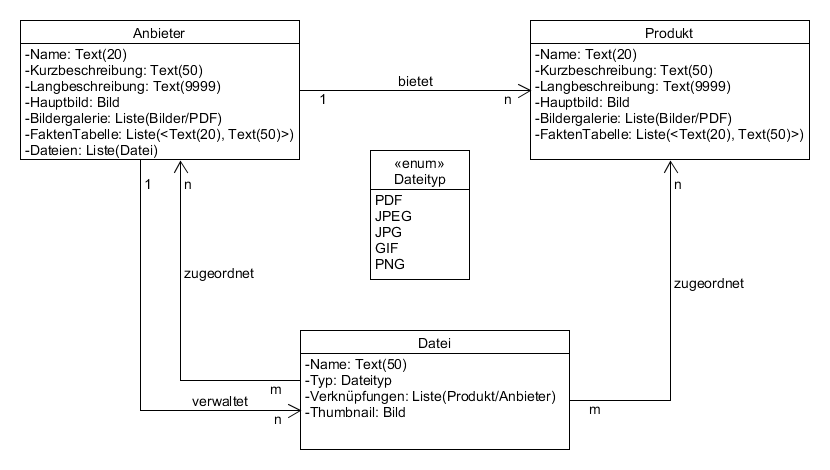
\includegraphics[width=1.0\textwidth]{FDM.png}
  \caption{Fachliches Datenmodell}
  \label{fig:fmd}
\end{figure}

\clearpage

\subsection{Benutzeroberfläche}

\begin{figure}[!htb]
  \centering
     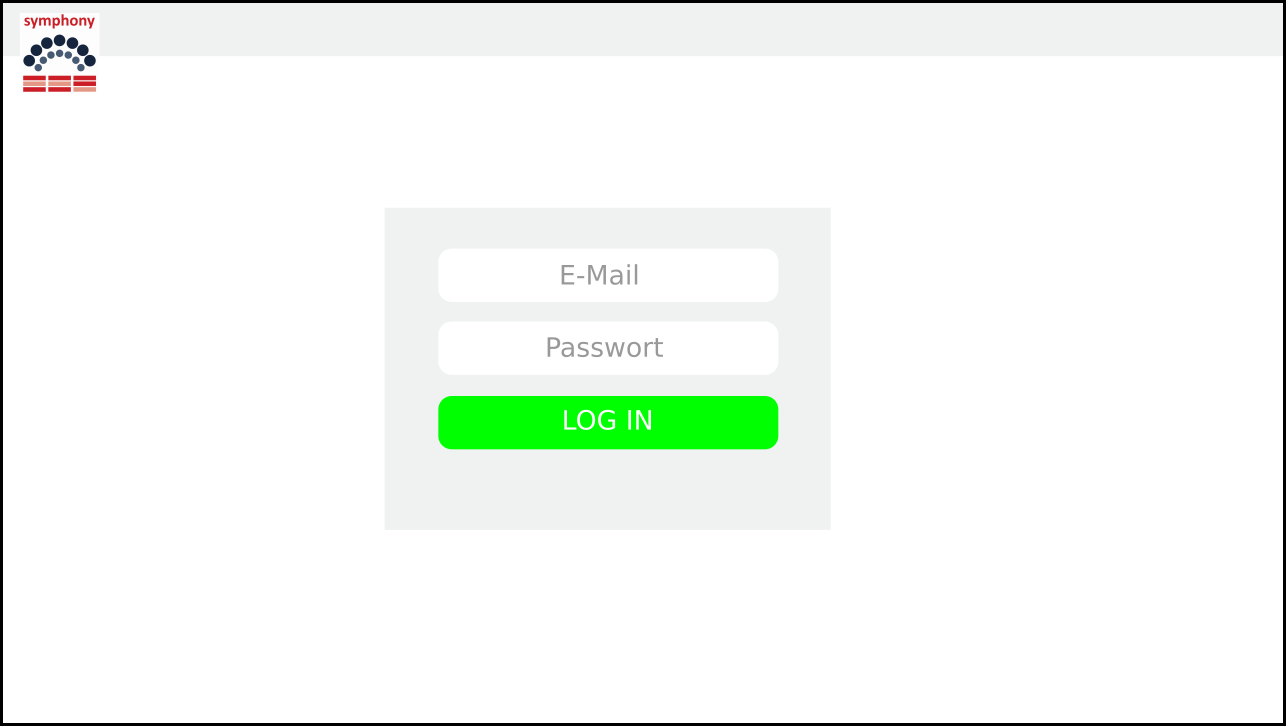
\includegraphics[width=1.0\textwidth]{projmicro_login.png}
  \caption{Login Mockup}
  \label{fig:login}
\end{figure}

\begin{figure}[!htb]
  \centering
     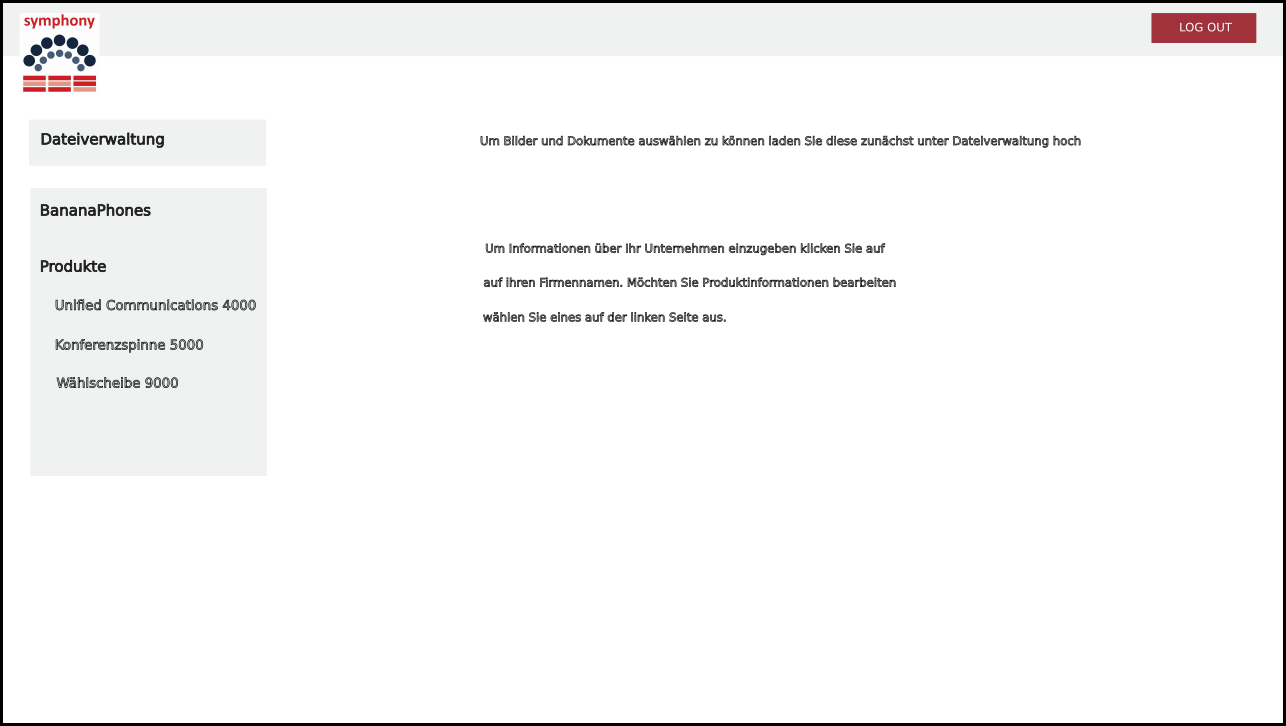
\includegraphics[width=1.0\textwidth]{projmicro_auswahl.png}
  \caption{Auswahlfenster Mockup}
  \label{fig:selection}
\end{figure}

\begin{figure}[!htb]
  \centering
     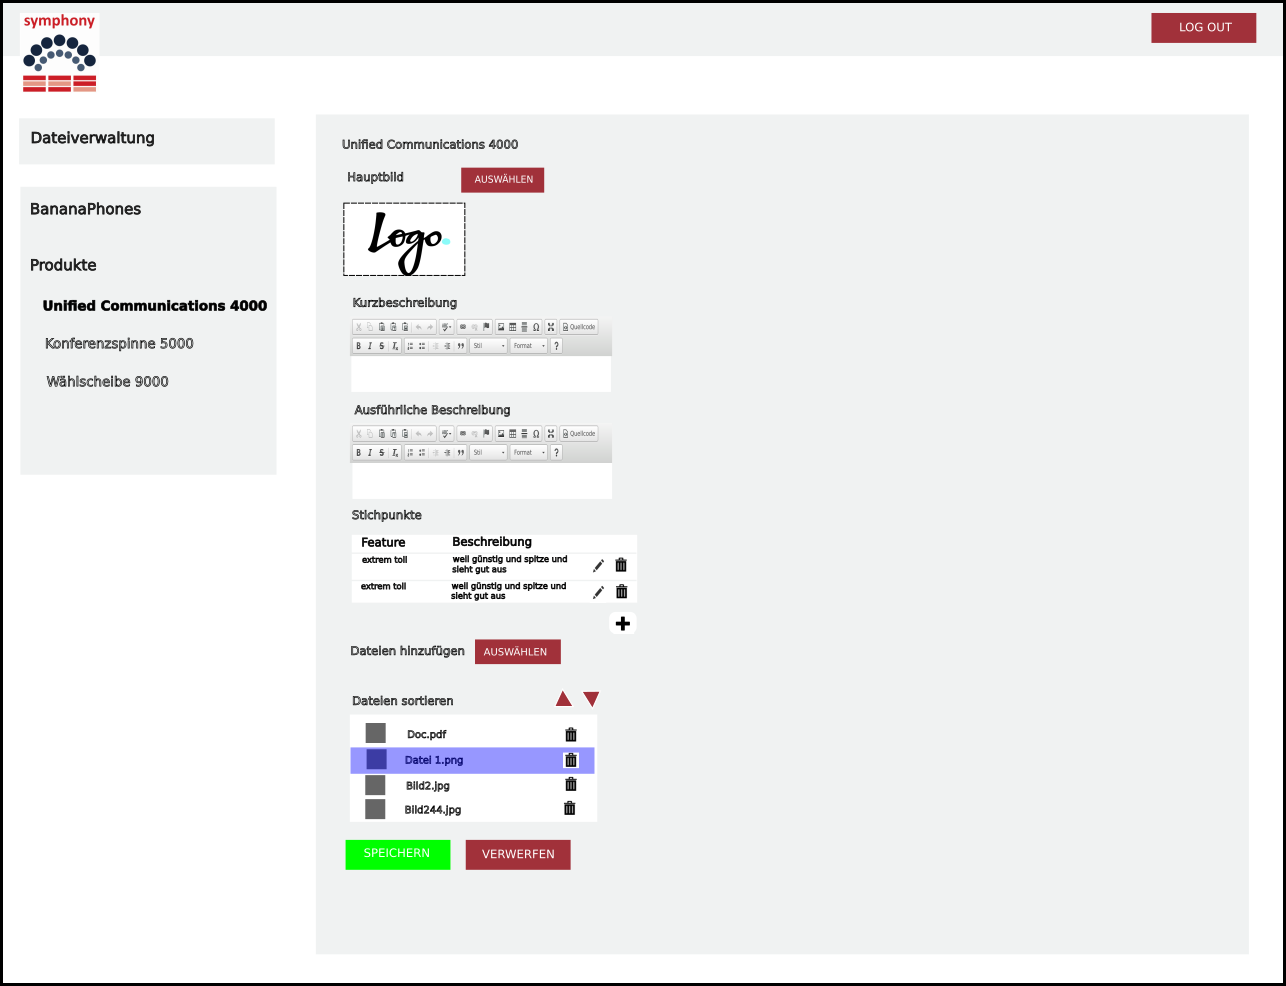
\includegraphics[width=1.0\textwidth]{projmicro_edit.png}
  \caption{Datensatz Bearbeitungs Mockup}
  \label{fig:edit}
\end{figure}

\begin{figure}[!htb]
  \centering
     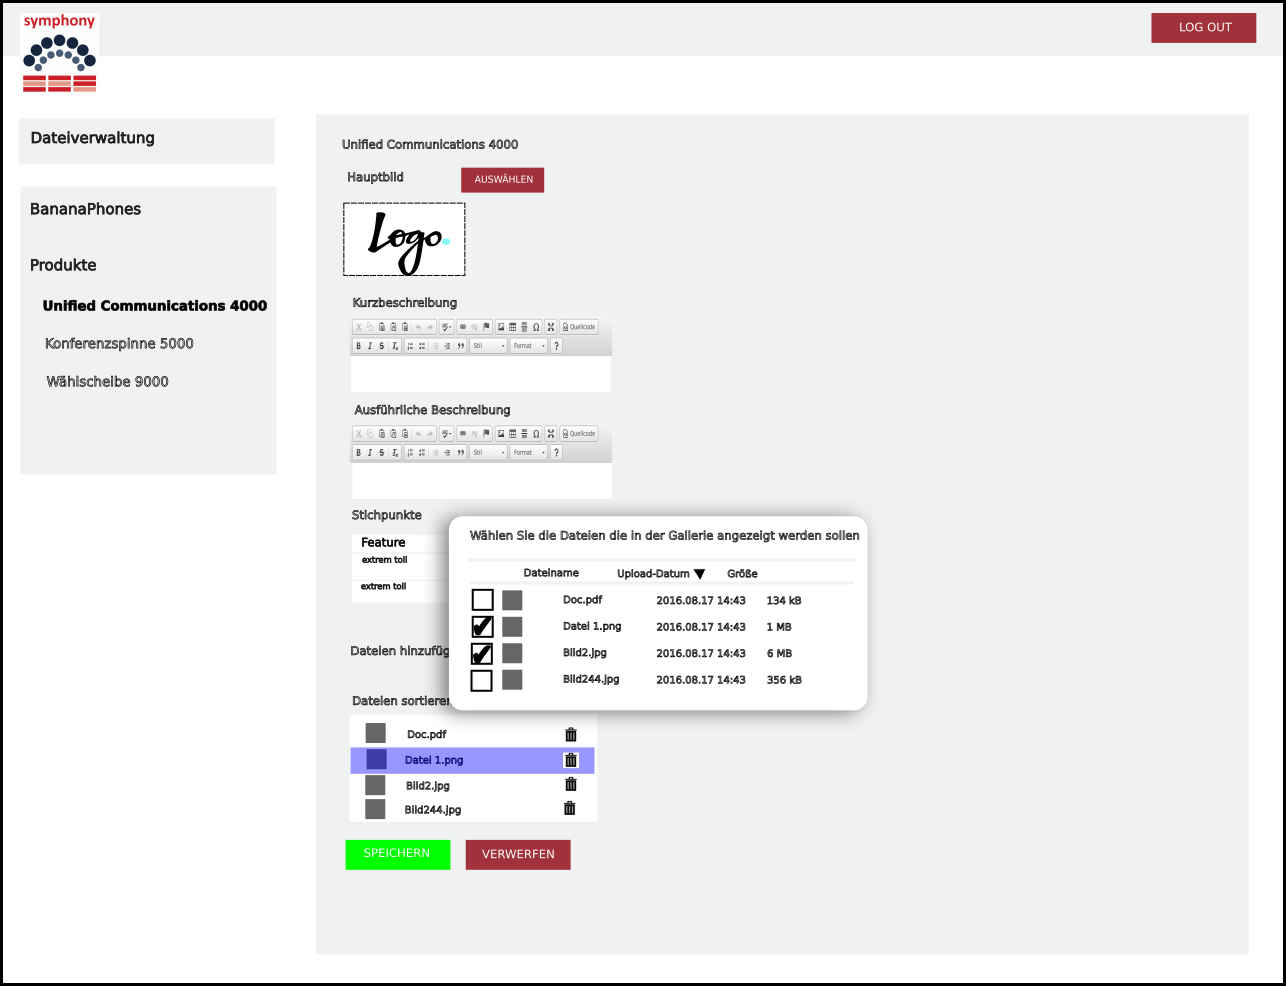
\includegraphics[width=1.0\textwidth]{projmicro_edit_dateiauswahl.png}
  \caption{Datensazu Bearbeitungs Mockup mit Upload}
  \label{fig:edit_file}
\end{figure}

\begin{figure}[!htb]
  \centering
     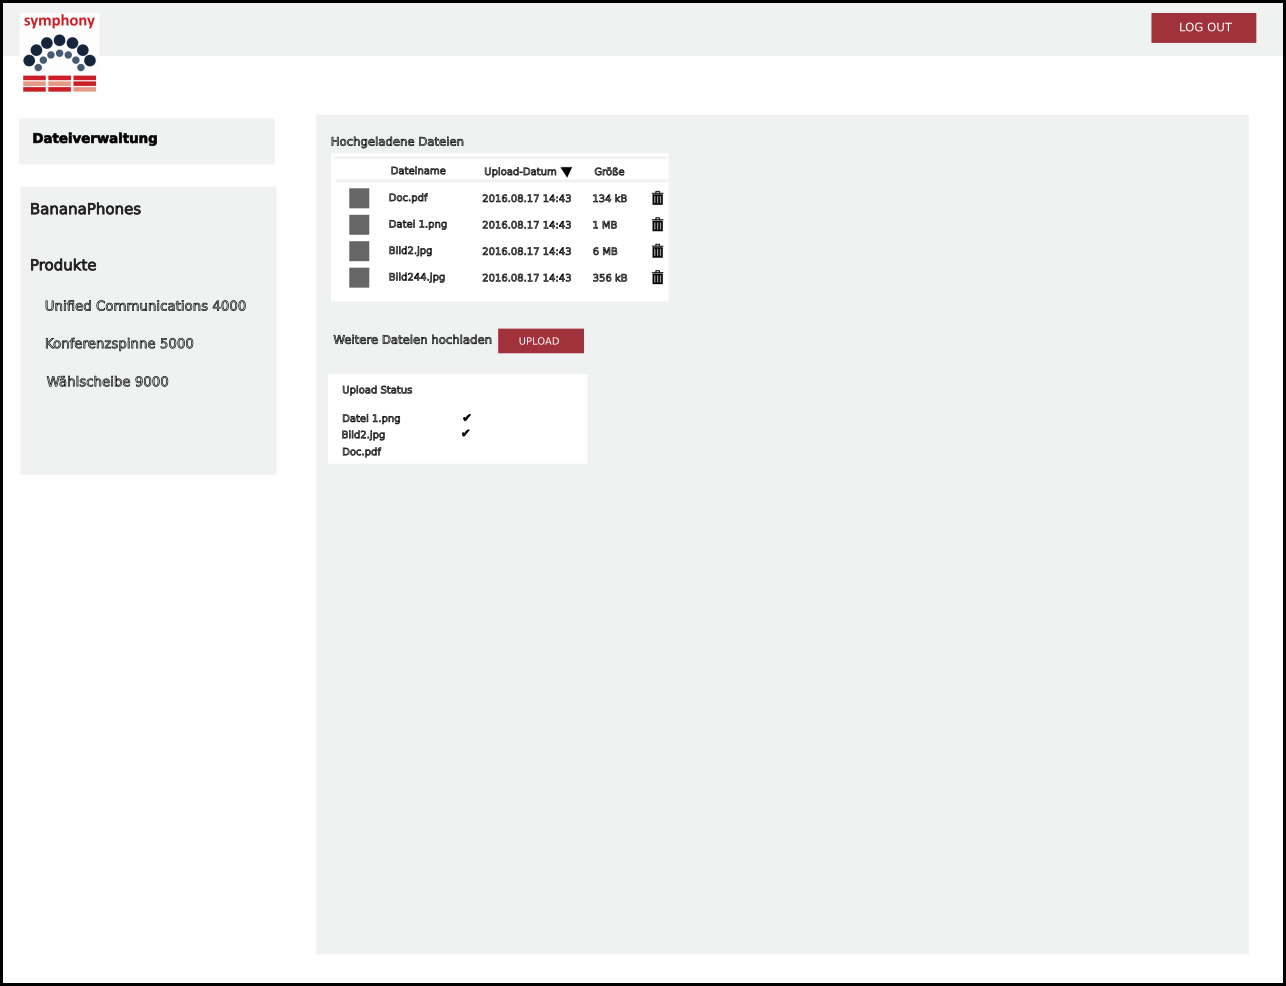
\includegraphics[width=1.0\textwidth]{projmicro_upload.png}
  \caption{Dateiverwaltung Mockup}
  \label{fig:selection}
\end{figure}

\section{Entwicklungsumgebung}
Da das Projekt ein Gradle Projekt ist, wird grundsätzlich nur eine IDE benötigt, die Gradle Projekte unterstützt.
In der Entwicklungsphase wurde IntelliJ IDEA 2016.2.4 genutzt. Weiterhin wurde das Java SDK in der Version 1.8 genutzt.
Die Datenbank ist eine embedded Mongo DB.
Zusätzliche Abhängigkeiten werden über Gradle Dependencies aufgelöst.

\clearpage

%%%%%%%%%%%%%%%%%%%%%%%%%%%%%%%%%%%%%%%%%%%%%%%%%%%%%%%%%%%%%%%%%%%%%%
% Begriffslexikon zur Beschreibung des Produkts						 %
%%%%%%%%%%%%%%%%%%%%%%%%%%%%%%%%%%%%%%%%%%%%%%%%%%%%%%%%%%%%%%%%%%%%%%
\newglossaryentry{sortierschluessel}
{
  name=Sortierschlüssel,
  description={ein Schlüssel, anhand dessen diese Einträge sortiert werden}
}
\newglossaryentry{bananarama}
{
  name=Bananarama,
  description={ein zweiter Eintrag}
}
\newglossaryentry{lorem}
{
  name=Lorem Ipsum,
  description={ein Blindtext}
}
\newacronym{abc}{Blub}{Bananarama}

% Setze den richtigen Namen für das Glossar
\renewcommand*{\glossaryname}{\section{\glossarName}}

% Drucke das gesamte Glossar
\glsaddall
\printglossaries

% Trage das Glossar in das Inhaltsverzeichnis ein
\stepcounter{section}
\addcontentsline{toc}{section}{\numberline {\thesection} \glossarName}


\end{document}
